
\paragraph{Semaforo privo di enable}
Per la realizzazione una FSM che alterni gli stati come in \figurename{\ref{fig:stati}}
Avendo tre stati diversi è stato necessario impiegare una codifica a 2 bit.
Essendo la codifica arbitraria si riporta la codifica impiegata in
\tablename{\ref{tab:cod}}.
Essendo possibile con due bit ottenere anche lo stato 11,  non corrispondente a nessuno degli stati codificati,
è stato imposto che dallo stato ROSSO sul successivo fronte di salita di clock il segnale costituisca
un reset forzando pertanto la transizione \\ROSSO $(1;0)$  $\longrightarrow$ VERDE $(0;0)$.
Rendando pertanto il lo stato 1;1 quale inaccessibile.
Si riporta la \tablename{ \ref{tab:tran}} delle transizioni tra i vari stati della FSM.

Dalla \tablename{ \ref{tab:tran}} si ottiene  $b_{1}^{n+1} = \overline{b_{1}^{n}} \cdot b_{0}^{n}$ e $b_{0}^{n+1} = \overline{b_{1}^{n}} \cdot \overline{b_{0}^{n}}$
\\
\\
SCRIVERE CHE TIPO DI MACCHINA é
\\
\\
Per realizzare la FSM basata sugli integrati a disposizione, e che realizzi quanto appena descritto,
 è stato realizzato il circuito in \figurename{ \ref{fig:sem1}} alimentando la componentistica con una tensione
 $V_{cc}=$\SI{0.1 \pm 456456215}{\volt}.Si segnala inoltre che in serie con i led sono state montate delle resistenze $R\sim 330$\si{\ohm} per limitare la richiesta di corrente.
\begin{figure}[h!]
	\begin{minipage}{0.5\textwidth}
		\centering
		\includegraphics[scale=0.20]{immagineM.png}
		\caption{Stati della FSM semaforo senza En.}
		\label{fig:stati}
	\end{minipage}
\begin{minipage}{0.5\textwidth}
	\centering
	\begin{tabular}{ssc}
	\toprule
	b_{1} & b_{0} & stato corrispondente\\
	\midrule
	0 & 0 & VERDE\\
	0 & 1 & GIALLO \& VERDE\\
	1 & 0 & ROSSO\\
	1 & 1 &  X (NON VOLUTO)\\
	\bottomrule
	\end{tabular}
	\caption{Codifica degli stati impiegati}
	\label{tab:cod}
\end{minipage}
\end{figure}


\begin{table}[h]
\centering
\begin{tabular}{ss|ss|sss}
	\toprule
	b_{1}^{n} & b_{0}^{n}  & b_{1}^{n+1} & b_{0}^{n+1} & \text{LED VERDE} & \text{LED GIALLO} & \text{LED ROSSO} \\
	\midrule
	 1 & 1 & 0 & 0 & x & x& x\\
	 0 & 1 & 1 & 0 & 1 & 1& 0\\
	 1 & 0 & 0 & 0 & 0 & 0& 1\\
	 0 & 0 & 0 & 1 & 1 & 0& 0\\
	\bottomrule
\end{tabular}
\caption{Tabella delle transizioni della FSM semaforo sempre abilitato.
Il segnale $1$ corrisponde al LED acceso, $0$ LED spento.
Lo stato $b_{1}=1$ $b_{0}=1$ deve risultare inaccessibile. }
\label{tab:tran}
\end{table}

\begin{figure}[h!]
		\centering
		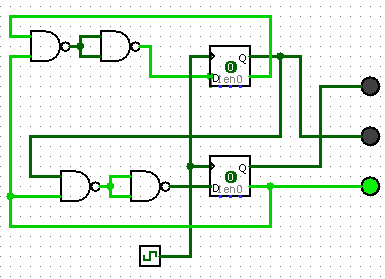
\includegraphics[scale=1.0]{circ1.png}
		\caption{Circuito che realizzi il semaforo senza En.}
		\label{fig:sem1}
	\end{figure}

Per la verifica del funzionamento circuitale è stato
 inviato un segnale di clock di frequenza bassa, $f\sim $\si{\hertz} e effettuando un primo controllo attraverso l'accensione dei LED. Si è successivamente aumentata la frequenza di clock $f= $\SI{.0000001\pm 45}{\hertz}
 ed acquisito i valori di tensione corrispondente alle uscite dei vari LED, riportate in
 \figurename{ \ref{fig:acq}}. Dall'osservazione di
  tali acquisizioni si verifica l'accordo con le specifiche attese.

\begin{figure}[h]
	\centering
	\subfloat[clock ch.  LED VERDE ch]{
		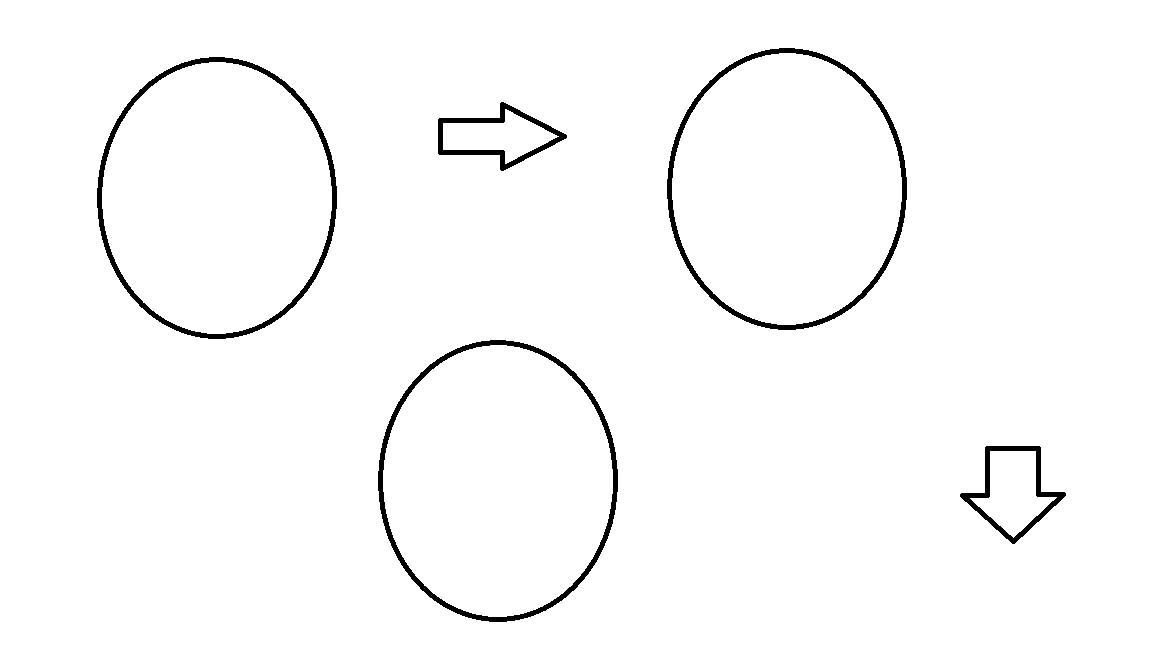
\includegraphics[scale=0.3]{Immagine.png}
	}
	\subfloat[clock ch. LED GIALLO ch]{
		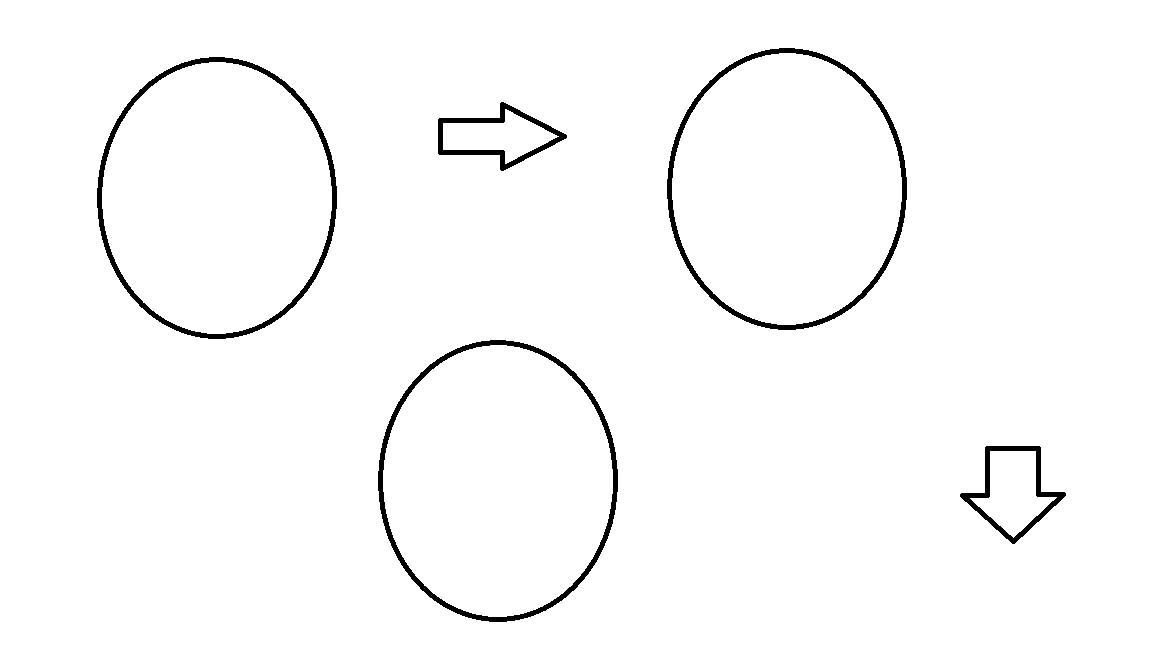
\includegraphics[scale=0.3]{Immagine.png}
		}\\
	\subfloat[clock ch.  LED ROSSO ch]{
		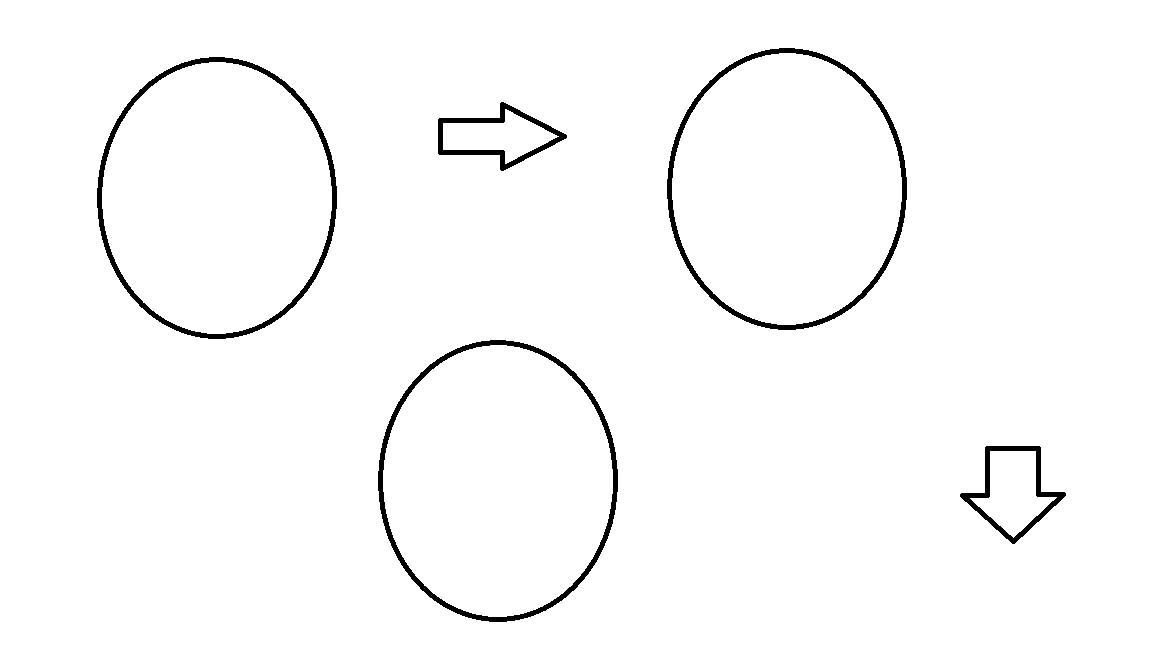
\includegraphics[scale=0.3]{Immagine.png}
		}
	\subfloat[clock ch.  $b_{0}$ ch]{
		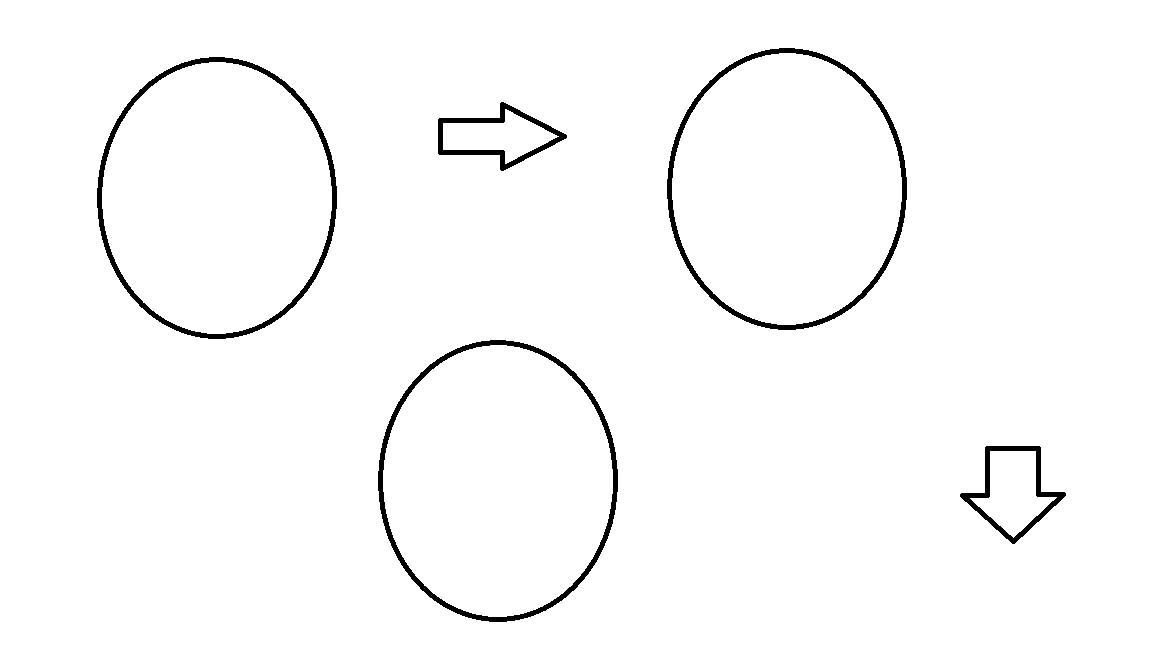
\includegraphics[scale=0.3]{Immagine.png}
		}\\
	\subfloat[clock ch. $b_{1}$  ch]{
		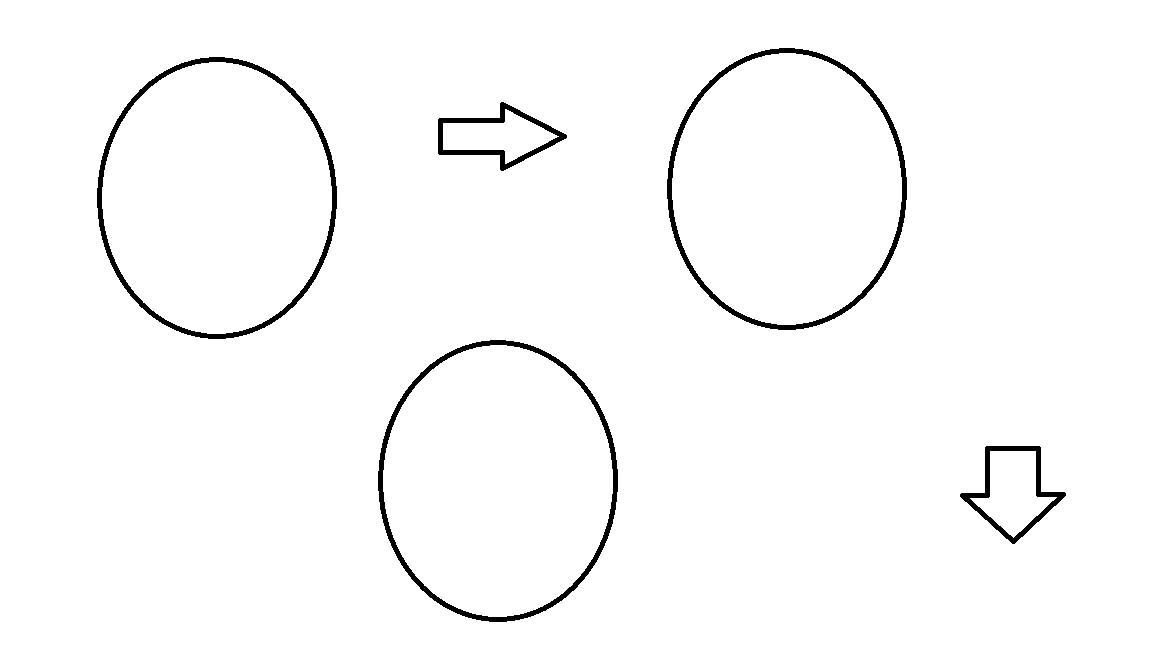
\includegraphics[scale=0.3]{Immagine.png}
	}
\caption{Acquisizione telle tensioni osservate nel semaforo privo di ENABLE}
\label{fig:acq}
\end{figure}
